%%% Choose between 16:9 and 4:3 format by commenting out/uncommenting one of the following lines:
\documentclass[aspectratio=169]{beamer} % 16:9
% \documentclass{beamer} % 4:3

%=========================================================================================================================
\usepackage[ngerman]{babel}
\usepackage[utf8]{inputenc}
% \usepackage[english]{babel}     % English language
\usepackage[latin1]{inputenc}   % Input encoding
\usepackage{tikz}               % For creating graphics
\usepackage{ulem} % für das Unterstreichen
\usepackage{url}                % For including urls
\usepackage{tabularx}           % For better tables
\usepackage{graphicx}
\usetheme{aig}                  % Set beamer theme
\usepackage{enumitem}
\documentclass{article}

\usetikzlibrary{arrows.meta, positioning, shapes.geometric}

\usepackage{xcolor} %  use colors

\definecolor{myred}{rgb}{1, 0, 0}
\definecolor{myblue}{rgb}{0, 0, 1}
\definecolor{mygreen}{rgb}{0, 1, 0}
\definecolor{mypurple}{rgb}{0.5, 0, 0.5}
\definecolor{myorange}{rgb}{1, 0.5, 0}
\definecolor{mypink}{rgb}{1, 0.75, 0.8}
\definecolor{mycyan}{rgb}{0, 1, 1}
\definecolor{mybrown}{rgb}{0.6, 0.4, 0.2}
\definecolor{mygelb}{rgb}{1.0, 1.0, 0.0}  


%=========================================================================================================================
\title{Erkennung von Hate Speech mit Twitter - Zwischenpr\"asentation}

\author[Friedrich, Tuychieva, Wall, Chalil, Engels]{Elena Marion Friedrich, Nasiba Tuychieva, Sven Ole Wall, Imran Nteli Chalil, Christian Engels}
\institute{Artificial Intelligence Group,\\
University of Hagen, Germany}
\date{17. Dezember 2024}
%=========================================================================================================================
\logo{\includegraphics[width=3cm]{figures/logoaig.png}}
%=========================================================================================================================

\begin{document}

%=========================================================================================================================

\begin{frame}
  \titlepage
\end{frame}
\nologo

\begin{frame}
		\frametitle{Overview}
        \tableofcontents[]
\end{frame}

\section{Fragestellung}
\begin{frame}{Fragestellung}
    \begin{block}{Ausgangsfrage}
        Wie kann mithilfe von klassischen Verfahren des maschinellen Lernens sowie mit Deep-Learning-Verfahren Hate Speech auf sozialen Plattformen anhand des Beispiels Twitter erkannt werden?
        \begin{itemize}
            \item Klassifikation von Text / Sentiment Analysis
        \end{itemize}
    \end{block}    
\end{frame}


\section{Workflow}
\begin{frame}{Workflow}
 \begin{figure}[h!]
        \centering
        \includegraphics[scale=0.5]{figures/workflow_latestV.png}
        %\caption{Workflow}
        \label{fig:yourimage}
    \end{figure}
\end{frame}
%\begin{frame}{Workflow}
% \begin{figure}[h!]
%        \centering
%        \includegraphics[scale=0.7]
%{figures/workflow_neu.png}
 %       %\caption{Workflow}
%        \label{fig:yourimage}
%    \end{figure}
%\end{frame}


\section{Close-up: Datenbereinigung}

\begin{frame}{Close-up: Datenbereinigung}
    \begin{itemize}[label=\textbullet]
        \item \textcolor{myred}{Entfernung unnötiger Zeichen}  
        \item \textcolor{myblue}{Entfernung von Erwähnungen}
        \item \textcolor{myorange}{Auftrennen zusammengeschriebener Wörter}
        \item \textcolor{mygreen}{Entfernung von Stopwords und häufigsten Wörtern}
        \item \textcolor{mypurple}{Konvertierung von Emojis zu Text}
        \item \textcolor{mybrown}{Stemming und Lemmatisierung}
    \end{itemize}

     \begin{columns}[T] % Aligns the top of the columns
        \begin{column}{0.5\textwidth}
            \begin{enumerate}[label=\arabic*.] 
                %\item marble #balloons just make me extremelly %\textcolor{myred}{!} 
                %\colorbox{mypurple}{\includegraphics[width=0.3cm]
                % {figures/grinning.png}} 
                %\colorbox{mypurple}{\includegraphics[width=0.3cm]
                % {figures/balloon.png}} \textcolor{myred}{\#}lazysaturday 
                % \textcolor{myred}{\#}home 
                % \textcolor{myred}{\#}tattoo 
                % \textcolor{myred}{\#}pineapple 
                % \textcolor{myred}{\#}beautiful
                \item \textcolor{myred}{\#}\textcolor{myorange}{national}\textcolor{mybrown}{best}\textcolor{myorange}{friend}\textcolor{mybrown}{s}\textcolor{myorange}{day}
                \textcolor{myred}{\#}\textcolor{mybrown}{sisters}
                \textcolor{myred}{\#}family 
                \textcolor{myred}{\#}love thank 
                \textcolor{mygreen}{you}
                \textcolor{myblue}{@user} 
                \textcolor{mygreen}{for being my} 
                \textcolor{mybrown}{best} friend 
                \colorbox{mypurple}{\includegraphics[width=0.3cm]{figures/heart.png}} 
                \colorbox{mypurple}{\includegraphics[width=0.3cm]{figures/grinning.png}} 

                % \item super fun 
                % \textcolor{mygreen}{with} 
                % \textcolor{mygreen}{my} 
                % \textcolor{mypink}{best} 
                % \textcolor{mygreen}{in} ideacity 
                % \textcolor{myred}{\#}zoomer 
                % \textcolor{myred}{\#}toronto 
                % \textcolor{myred}{\#}life 
                % \textcolor{myred}{\#}love 
                % \textcolor{myred}{\#}
                % \textcolor{mybrown}{friends} 
                % \textcolor{myblue}{@zoomerplex}
                \item \textcolor{myblue}{@user} 
                \textcolor{mygreen}{i will be there} 
                \textcolor{myred}{!!!} 
                \textcolor{mybrown}{hoping} 
                \textcolor{mygreen}{for a} beautiful day \(  \sim  \)  clear \textcolor{mybrown}{skies} 
                \textcolor{mygreen}{with a} breeze would 
                \textcolor{mygreen}{be} perfect 
                \textcolor{myred}{!!! ;)} 
            \end{enumerate}
        \end{column}
        \begin{column}{0.5\textwidth}
            \begin{enumerate}[label=\arabic*.] 
                %\item marble balloons just make me extremelly %\textcolor{mypurple} {beaming face with smiling eyes 
                % balloon} lazysaturday home tattoo pineapple beautiful
                \item 
                \textcolor{myorange}{national} 
                \textcolor{myorange}{go}\textcolor{mybrown}{od} 
                \textcolor{myorange}{fri}\textcolor{mybrown}{end} 
                \textcolor{myorange}{day}
                \textcolor{mybrown}{sister} family love thank friend 
                \textcolor{mypurple}{sparkle heart grinning face}
                % \item super fun 
                % \textcolor{mypink}{good} toronto life 
                % \textcolor{mybrown}{friend}
                \item \textcolor{mybrown}{hope} beautiful day \(  \sim  \) clear 
                \textcolor{mybrown}{sky} breeze would perfect
            \end{enumerate}
        \end{column}
    \end{columns}
\end{frame}


\section{Close-up: Vektorisierung}
\begin{frame}{Close-up: Vektorisierung}
    %\begin{itemize}[label=\textbullet]
    %    \item Zunächst 4 Vektorisierungsmethoden: BoW, TF-IDF, W2V, Fasttext
    %   \item Nach Literaturrecherche Einigung auf TF-IDF, W2V und Glove 
    % (mit 200d Twitterdateien geladen)
    %    \item Funktionen als python Datei zur Verfügung gestellt
    %    \item Funktionen evalutiert (s.u.):
    %    \item Versuche mit W2V Parametern (min\_count, window, vector\_size)
    %\end{itemize}
    \begin{figure}[h!]
        \centering
        \includegraphics[scale=0.8]{figures/nb_vectorize_functions.png} % original: scale=0.6
        %\caption{Mit NB evaluierte Vectorize Functions}
        \label{fig:yourimage}
    \end{figure}
\end{frame}


% Nasiba
\section{Close-up: Datenexploration}

\begin{frame}{Close-up: Datenexploration}
\begin{figure}[ht]
    \centering
    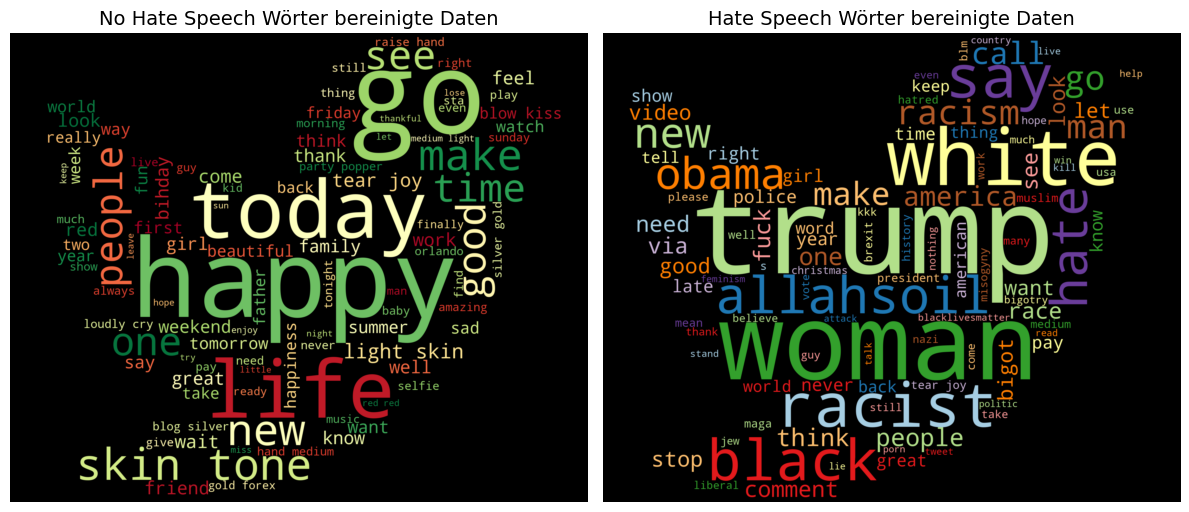
\includegraphics[width=\textwidth]{figures/nohate_hate_speech.png} % Bildbreite angepasst
    \caption{No Hate Speech und Hate Speech Tweets } 
    \label{fig:meinbild}
\end{figure}
\end{frame}

\section{Besonderheiten des Datensatzes}
\begin{frame}{Besonderheiten des Datensatzes}
% Set margins
    \begin{minipage}[t][0.9\textheight][t]{0.28\textwidth}
        % First rectangle
        \vspace{0.6cm} % top margin
        \textbf{Binäre Klassifizierung (nur Trainingsdaten)}
        \vspace{0.75cm} % empty row after title
        \\
        Labels unterscheiden zwischen Hassrede und Nicht-Hassrede
        \\
        [1.45cm]
        %\vspace{0.7cm}
        \textrightarrow\ Auswahl der Algorithmen und Metriken 
    \end{minipage}
\end{frame}


\begin{frame}{Besonderheiten des Datensatzes}
% Set margins
    \begin{minipage}[t][0.9\textheight][t]{0.28\textwidth}
        % First rectangle
        \vspace{0.6cm} % top margin
        \textbf{Binäre Klassifizierung (nur Trainingsdaten)}
        \vspace{0.75cm} % empty row after title
        \\
        Labels unterscheiden zwischen Hassrede und Nicht-Hassrede
        \\
        [1.45cm]
        %\vspace{0.7cm}
        \textrightarrow\ Auswahl der Algorithmen und Metriken 
    \end{minipage}
    \hspace{0.5cm}
    \begin{minipage}[t][0.9\textheight][t]{0.28\textwidth}
        % Second recangle
        \vspace{0.6cm} % top margin
        \textbf{Unausgeglichener Datensatz}
        \vspace{0.35cm} % empty row after title
        \begin{itemize}[label=\textbullet]
            \item 29720 Datensätze Nicht-Hassrede
            \item 2242 Datensätze Hassrede 
        \end{itemize}
       % (unbereinigter Trainingsdatensatz)
        \\[1cm]
        \vspace{1cm}
        \\
        \textrightarrow\ Verzerrte Modelle und Metriken
    \end{minipage}
    \hspace{0.5cm}
\end{frame}

\begin{frame}{Besonderheiten des Datensatzes}
% Set margins
    \begin{minipage}[t][0.9\textheight][t]{0.28\textwidth}
        % First rectangle
        \vspace{0.6cm} % top margin
        \textbf{Binäre Klassifizierung (nur Trainingsdaten)}
        \vspace{0.75cm} % empty row after title
        \\
        Labels unterscheiden zwischen Hassrede und Nicht-Hassrede
        \\
        [1.45cm]
        %\vspace{0.7cm}
        \textrightarrow\ Auswahl der Algorithmen und Metriken 
    \end{minipage}
    \hspace{0.5cm}
    \begin{minipage}[t][0.9\textheight][t]{0.28\textwidth}
        % Second rectangle
        \vspace{0.6cm} % top margin
        \textbf{Unausgeglichener Datensatz}
        \vspace{0.35cm} % empty row after title
        \begin{itemize}[label=\textbullet]
            \item 29720 Datensätze Nicht-Hassrede
            \item 2242 Datensätze Hassrede 
        \end{itemize}
       % (unbereinigter Trainingsdatensatz)
        \\[1cm]
        \vspace{1cm}
        \\
        \textrightarrow\ Verzerrte Modelle und Metriken
    \end{minipage}
    \hspace{0.5cm}
    \begin{minipage}[t][0.9\textheight][t]{0.28\textwidth}
        % Third rectangle
        \vspace{0.6cm} % top margin
        \textbf{Verwendete Sprache}
        \vspace{0.35cm} % empty row after title
        \vspace{0.35cm} % empty row after title
        \begin{itemize}[label=\textbullet]
            \item Rechtschreibfehler
            \item Abkürzungen
            \item Emoticons
            \item @-Erwähnungen
            \item Hashtags
        \end{itemize}
        \\
        \vspace{0.3cm}
        \textrightarrow\ Beeinflussung der Modellgenauigkeit
        \\\Rightarrow\ \text{ Vorverarbeitung}
    \end{minipage}
\end{frame}


\section{Verfeinerung Fragestellung}
\begin{frame}{Verfeinerung Fragestellung}
    \begin{block}{Ausgangsfrage}
        Wie kann mithilfe von klassischen Verfahren des maschinellen Lernens sowie mit Deep-Learning-Verfahren Hate Speech auf sozialen Plattformen anhand des Beispiels Twitter erkannt werden?
        \begin{itemize}
            \item Klassifikation von Text / Sentiment Analysis
        \end{itemize}
    \end{block}    
    \begin{exampleblock}{Methodische Detailfragen}
        \begin{itemize}
            \item Welche M\"oglichkeiten zum Umgang mit Klassenungleichgewichten gibt es und wie ist deren Einfluss auf die Modellperformance?
        \end{itemize}
    \end{exampleblock}
\end{frame}

\section{Ausblick: Model Training}
\begin{frame}{Ausblick: Model Training}
    \begin{itemize}[label=\textbullet]
            \item Naïve Bayes
            \item Support-Vektor-Maschine 
            \item Ensemble Learning
            \item RNN-LSTM
            \item RNN-GRU
    \end{itemize}
    
    \begin{figure}[h!]
        \centering
        \vspace{0.4cm}
        \includegraphics[scale=0.5]{figures/model_training2.png}
        %\caption{Model Training Workflow}
        \label{fig:yourimage}
    \end{figure}
\end{frame}


% \appendix

% \section{Appendix}

% \begin{frame}{Appendix}
%    This is an appendix.
%   \begin{itemize}
%       \item Page numbers start from the 
% beginning.
%    \end{itemize}
% \end{frame}


\begin{frame}
  \titlepage
\end{frame}
\nologo

\end{document}